\chapter{Some mathematics}\label{ch:group}


In this chapter I just want to show some ideas and notation in math that I am
not sure you have seen yet. {\it It is not crucially important that you understand
anything in this chapter deeply}, but I think it will help orient
yourself in this research to have some idea of what certain terms and symbols
mean, and how they are connected with each other and physics.

In each section, I tried to provide the minimum amount of knowledge that I think is
needed for later sections of the book. Therefore the sections are in no way
complete, and many facts will be stated without proof. To fully understand the
subject matter of each section likely requires you to take a class. Hopefully
these notes will at least help motivate those subjects. You will see some facts
that are important to learn, and their context in physics and other areas of
math.


\section{Preliminary ideas}

We want to discuss math in a fairly abstract way, in part because one of our
goals will be to look at generic mathematical structures. At the end of the book 
we will look at groups, structures that have only three characteristics. We will
 see that many math structures you've already encountered are examples of 
groups\footnote{In
general this is quite powerful, because if you know a fact about a group, and
you know further that a math structure is a group, you immediately know that
fact about that structure. We will not really leverage this power in this book;
I just want you to get acquainted with notation and ideas.}.
Hence we will need some notation that is agnostic to any particular math
structure.

To start, a {\it set}\index{set} is a collection of objects of
any kind, anything\footnote{This is technically wrong. It turns out that one has
to be very careful how a set is defined. Bertrand Russell was the first do
discover this; if you are interested in what can go wrong, look up 
Russell's\index{Russell's paradox}
paradox. For our purposes, this subtlety won't matter.}
you can think of. Everyone in the room you're in forms a set. The counting
numbers form a set. The symmetries of a ball form a set. We usually denote a set
with curly brackets
\begin{equation}
A=\{1,2,3,4\}.
\end{equation}
This means that $A$ is the set containing the numbers 1, 2, 3, and 4.
The things that the set contains are called {\it elements}\index{element}
or\index{member} {\it members}, and we indicate that, e.g. 1 is an element of
$A$ by writing
\begin{equation}
1\in A,
\end{equation}
which we read as ``1 is an element/member of the set $A$" or ``1 is in $A$".
If we want to refer to an arbitrary element $a$ of $A$, we write
\begin{equation}
a\in A,
\end{equation}
and if we want to say that $b$ is not a member of $A$, we write
\begin{equation}
b\notin A,
\end{equation}
The number of elements in a finite set is called its\index{cardinality}
{\it cardinality}. The cardinality of the set $A$ above is 4, and we write
\begin{equation}
  |A|=4.
\end{equation}
A {\it finite} set has a finite cardinality; otherwise it's an infinite set.

It is also useful to introduce an organizational hierarchy for sets. For
instance the set
\begin{equation}
  B=\{1,2,3,4,5,6\}
\end{equation}
is larger than $A$, but it contains $A$ entirely. We write
\begin{equation}
A\subset B.
\end{equation}
Talking about set logic is a good opportunity to introduce some more notation.
It is common to use $\Forall$ as shorthand for ``for all" or ``for any".
Since $A\subset B$, we know that $\Forall a\in A$ we must have $a\in B$.
To express that last idea, we write
\begin{equation}\label{eq:subsetIn}
a\in A\Rightarrow a\in B.
\end{equation}
The\index{set!empty} {\it empty set} $\emptyset$ is the set with nothing in it
at all. If a set has at least one element, it is\index{nonempty} {\it nonempty}.
From \equatref{eq:subsetIn} it follows that for any set $C$
\begin{equation}
\emptyset\subset C~~~~\text{and}~~~~C\subset C.
\end{equation}


\begin{example*}{}{}
  This example serves to introduce some notation for some infinite 
  sets you're likely already familiar with.
  \begin{enumerate}
    \item $\N$ is our symbol for the\index{number!natural} {\it natural
          numbers}, i.e. the infinite set
          $$ \N=\{1,2,3,...\}. $$
    \item $\Z$ represents the\index{integers} {\it integers}, i.e. the infinite
          set
          $$ \Z=\{...,-3,-2,-1,0,1,2,3,...\}. $$
    \item The\index{number!rational} {\it rational numbers} $\Q$ are the 
          infinite set of
          fractions formed using integers, of course not allowing 0 to be in the
          denominator. We write
          $$ \Q=\left\{\frac{m}{n} \suchthat  m,n\in \Z~\text{and}~n\neq0\right\}. $$
          In the above, s.t. is shorthand for the phrase ``such that".
    \item The\index{number!real} {\it real numbers} $\R$ include, in addition to the
          rationals, numbers that cannot be expressed as a fraction of integers.
          These include numbers like $\sqrt{2}$ as well as numbers like
          $e$ and $\pi$. It is a major digression to write $\R$ in set notation,
          whose construction is achieved canonically by starting with the rationals, 
          so we'll just leave it at that.
    \item Define $i\equiv\sqrt{-1}$. The\index{number!complex} {\it complex
          numbers} are an extension of the reals allowing for roots of negative
          numbers. It is given by
          $$ \C=\{x+iy \suchthat x,y\in\R \}. $$
          Given a complex number $z=x+iy$, its {\it complex
          conjugate}\index{complex conjugate} $z^*$ is defined by
          $$ z^*\equiv x-iy.$$
          Since you need two independent real numbers to describe a complex
          number, you can visualize complex numbers as lying in a plane. A
          measure of the ``size" of a complex number is its distance from 
          the origin or its {\it magnitude}. This is given by
          $$ |z| = \sqrt{zz^*} = \sqrt{x^2+y^2}. $$
    \item $\N\subset \Z \subset \Q \subset \R \subset \C$.
          
  \end{enumerate}
\end{example*}


We can introduce the notion of a function. A\index{function} 
{\it function} or\index{map} {\it mapping} $f$ between $X$ and $Y$ 
associates $\Forall x\in X$ a unique element $f(x)\in Y$. We 
write
\begin{equation}
f:X\to Y.
\end{equation}
Usually $X$ is called the\index{domain} {\it domain} 
and $Y$ is called the\index{codomain} {\it codomain}.
The\index{image} {\it image} or\index{range} {\it range}
is $f(X)$, i.e. the set of all values $f$
 maps to given the domain. Note $f(X)\subset Y$.

Next we classify a few different kinds of functions.
A function is\index{injection} {\it injective}
or\index{one-to-one} {\it one-to-one} if each element in $X$
maps to a different element in $Y$. We can express this symbolically as
\begin{equation}
 \Forall x_1,x_2\in X,~f(x_1)=f(x_2)\Rightarrow x_1=x_2.
\end{equation}
A\index{surjection} {\it surjective} or\index{onto} {\it onto} function 
maps to every possible element of the codomain $Y$. Symbolically,
\begin{equation}
 \Forall y\in Y,~\Exists x\in X \suchthat y=f(x), 
\end{equation}
where we have introduced the symbol $\Exists$ as shorthand for ``there is at
least one" or ``there exists". Finally a function is\index{function!bijective}
{\it bijective} if it is both an injection and a surjection. In this case each
element of $X$ corresponds to exactly one element of $Y$, and vice-versa.
Pictorial representations of these kinds of functions are shown in
\figref{fig:mapping}.

\begin{figure}
\centering
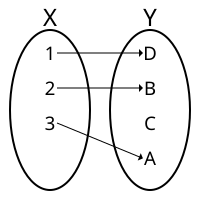
\includegraphics[width=0.45\linewidth]{figs/Injection.png}~~~
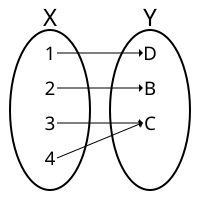
\includegraphics[width=0.45\linewidth]{figs/Surjection.png}\\
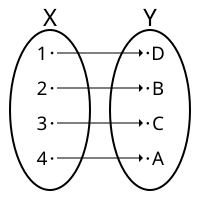
\includegraphics[width=0.45\linewidth]{figs/Bijection.png}~~~
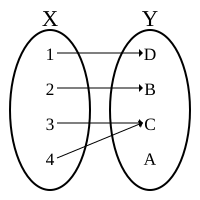
\includegraphics[width=0.45\linewidth]{figs/Not-Injection-Surjection.png}
\caption{Example mappings that are injective (top left), surjective (top right),
bijective (bottom left), and none of these (bottom right). Images taken from 
Wikipedia~\cite{wiki:bijection}.}
\label{fig:mapping}
\end{figure} 

Besides giving the opportunity to show some notation, one useful thing you can
do with bijections is use them to compare set cardinalities. Indeed, if you can
find a bijection $f$ between $X$ and $Y$, you know that $X$ and $Y$ have the
same size. While this is not particularly useful for finite sets, it is useful
for infinite sets, allowing one to classify various kinds of infinity.

\begin{example*}{}{}
Whenever you can find a bijection $f$ between any set $A$ and $\N$, $A$ is said to
be\index{countable} {\it countably infinite}. This infinity, the number
of natural numbers, is usually written\footnote{This symbol is pronounced
``aleph".} as $\aleph_0$, i.e.
$$|\N|=\aleph_0.$$
Intuitively the nomenclature ``countable" makes
sense, since you are using $f$ to assign a single counting number to each
element of $A$. What is perhaps less intuitive is that $\Z$ is countable, i.e.
$$|\Z|=|\N|.$$
So even though $\N$ is fully contained in $\Z$, they have the same size! To see
this, we just need a bijection between $\N$ and $\Z$. Here is one: map every odd
number in $\N$ to the non-negative integers, i.e.
$$ f(1)=0,~f(3)=1,~f(5)=2,~...$$
and so on. Map every even number to the negative integers, i.e.
$$ f(2)=-1,~f(4)=-2,~f(6)=-3,~...$$
etc. This mapping associates exactly one integer to one natural number and vice
versa. It works because it exploits the fact that both sets are infinite. One
can show $\Q$ is also countably infinite, although the mapping is a bit more
subtle\footnote{One can do it for the positive rationals 
by setting up a table where rows represent
numerators and columns denominators. The counting then traces a squiggly path
through the table.}. On the other hand,
$$|\R|>|\N|.$$
This was first shown by Cantor using his so-called ``diagonal argument", which
you can look up if you are interested. The cardinality of the reals is usually
written as $\frak{c}$ and is sometimes called\index{power of the continuum}
the {\it power of the continuum}. This name is extremely badass. It is also
interesting to see that there are, in this sense, different sizes of infinities.
You may sometimes hear people talk about the\index{continuum hypothesis} 
{\it continuum hypothesis}. This hypothesis posits that
there is no set whose cardinality lies between $\aleph_0$ and $\frak{c}$.
Finally we note that any infinity that is not $\aleph_0$ is called {\it
uncountable}\index{uncountable}. Hence we say $\R$ is uncountably infinite.
\end{example*}

\begin{figure}
  \centering
  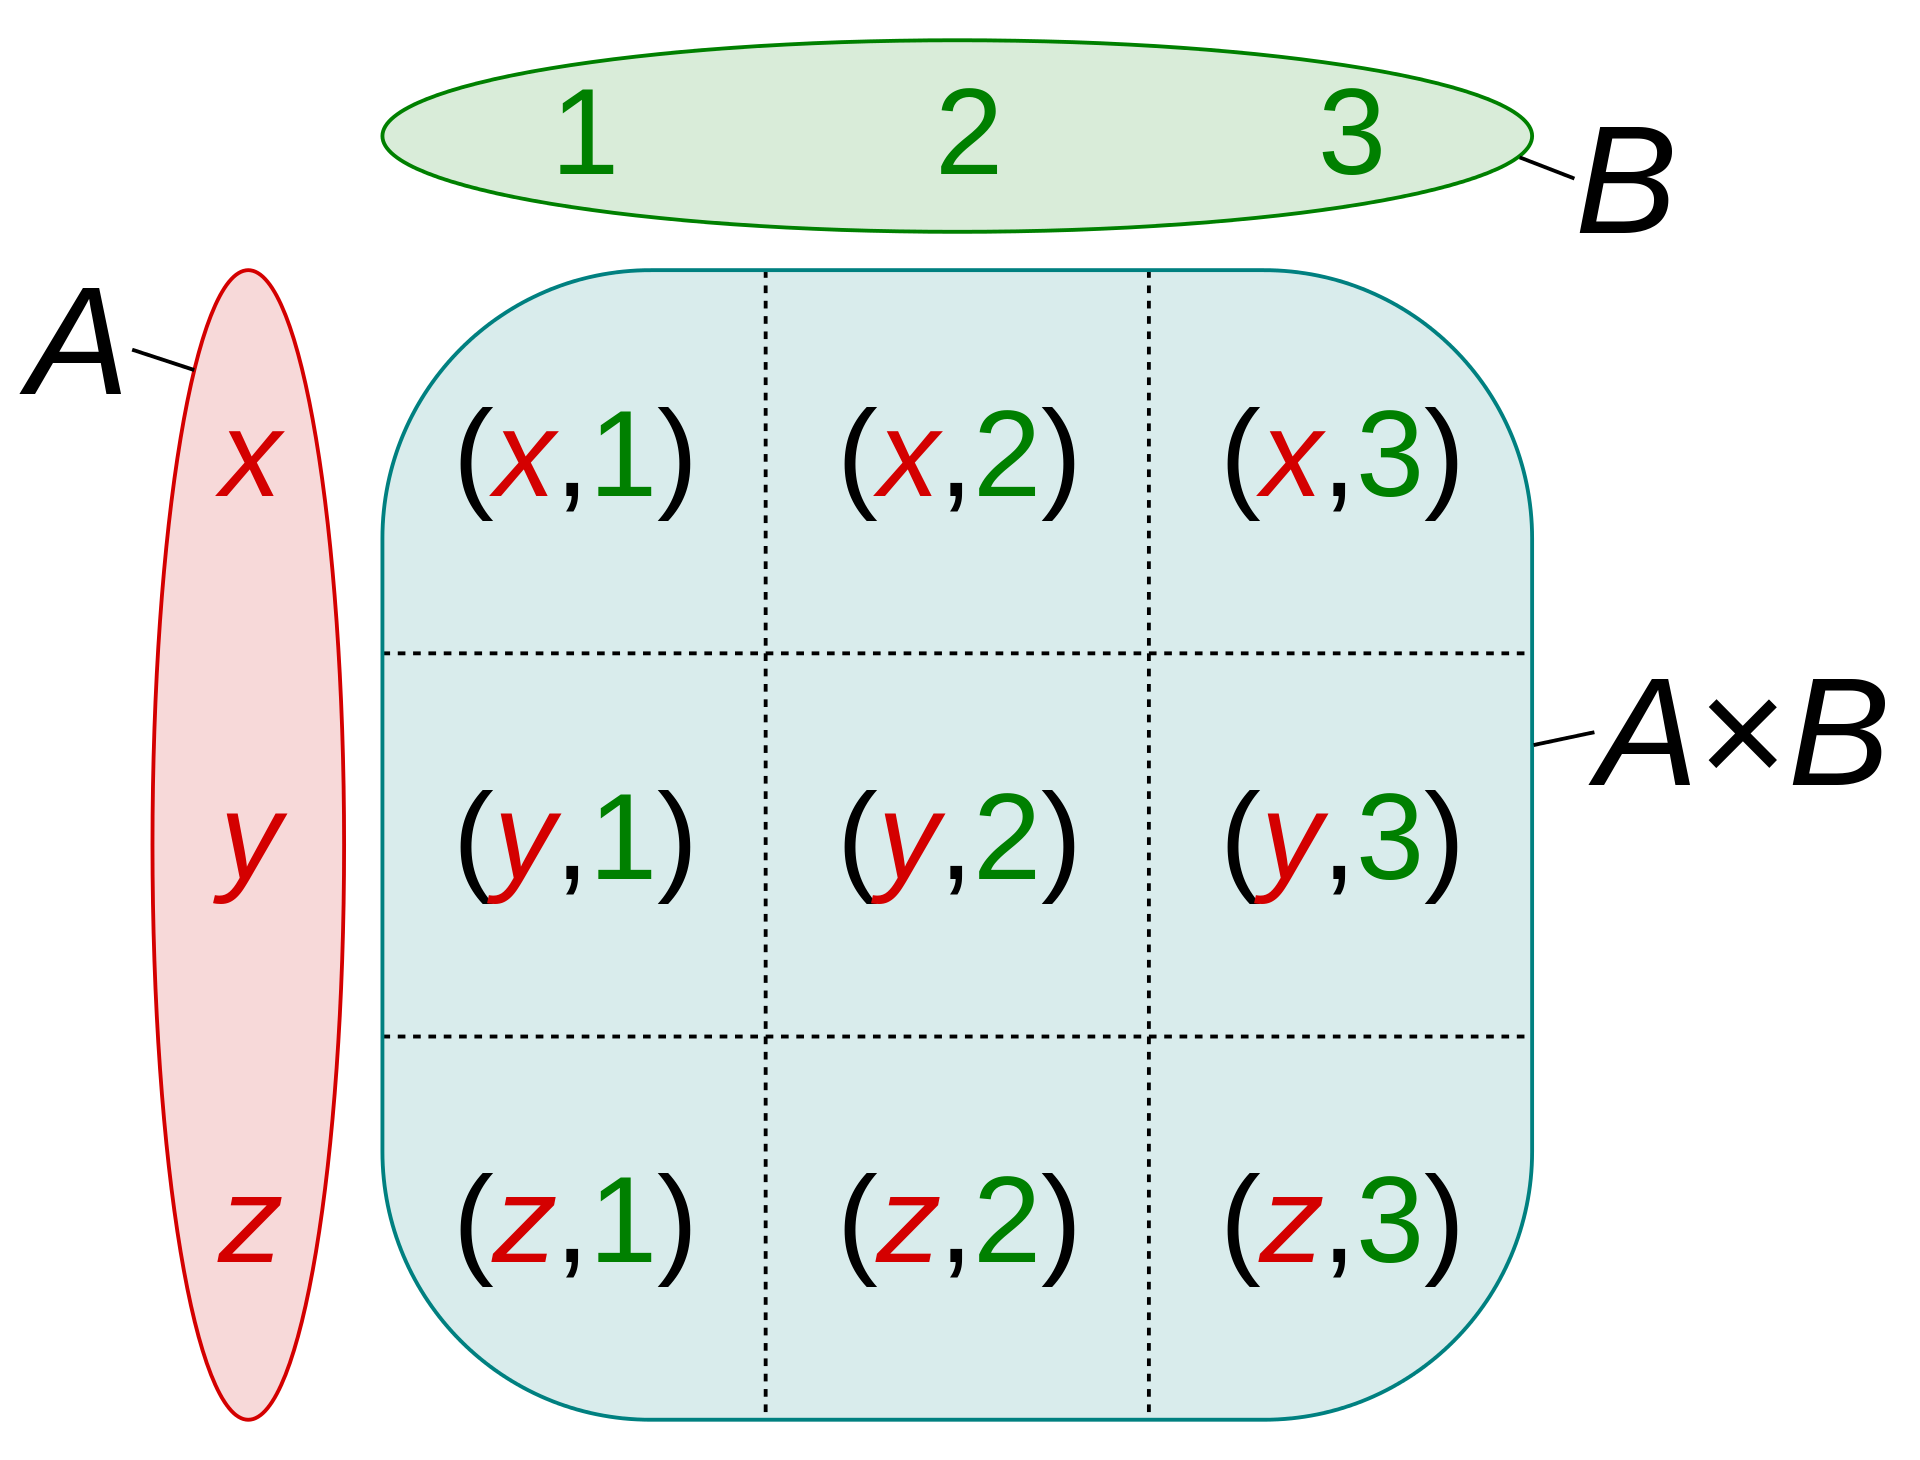
\includegraphics[width=0.45\linewidth]{figs/Cartesian_Product.png}~~~
  \caption{Example of a Cartesian Product. Image taken from 
  Wikipedia~\cite{wiki:cartesian_product}.}
  \label{fig:cartesian_product}
\end{figure} 

To close out the section, we discuss a couple ways of putting sets together.
The most straightforward way is just to ``add" the sets, i.e. form a new set
whose elements include all the elements from the parent sets. For instance if
you have two sets $A$ and $B$, then the\index{union} {\it union} is
\begin{equation}
A\cup B = \{x\suchthat x\in A~\text{or}~x\in B\}.
\end{equation}
You can also create that contains only the elements that both $A$ and $B$ have
in common. This set is the\index{intersection} {\it intersection}
\begin{equation}
A\cap B = \{x\suchthat x\in A~\text{and}~x\in B\}.
\end{equation}
We exist in nature in a space of more than one dimension; therefore it is useful to be
able to combine sets into coordinates. We define the\index{Cartesian product}
{\it Cartesian product} of $A$ and $B$ as the set of tuples
\begin{equation}
A\times B=\{(a,b)\suchthat a\in A~\text{and}~b\in B\}.
\end{equation}
See \figref{fig:cartesian_product} for a visual representation of the Cartesian
product. Later, we will use the Cartesian product to define multi-dimensional spaces.
For instance, a 4-$d$ space can be defined using the set 
\begin{equation}\label{eq:spacetimeSet}
\R^4\equiv\R\times\R\times\R\times\R=\{(x_0,x_1,x_2,x_3)\suchthat
x_0,x_1,x_2,x_3\in\R\}.
\end{equation}


\section{Vectors and matrices}\label{sec:vecmat}

In the last section we looked at many math objects that can be represented by a
single number. If $x\in\Q,\R$, or $\C$, we call\footnote{For this definition of scalar,
we won't let $x\in\N$ or $x\in\Z$ because in nature, we need the number 0 and want to
be able to divide sensibly.} $x$ a\index{scalar} {\it scalar}. 
Thinking ahead to physics, we can express many measurable quantities in nature
as scalars, for instance the temperature.

Some quantities also need to be represented with a direction, quantities such as
the gravitational force. To accomplish that we introduce a tuple of length $n\in\N$,
\begin{equation}\label{eq:vecDef}
  v=\colvec{4}{v_1}{v_2}{\vdots}{v_n},
\end{equation}
where the $v_i$, $1\leq i\leq n$, are scalars all belonging to the same set $A$, i.e.
\begin{equation}
  v\in \underbrace{A\times A\times ... \times A}_{n\text{ times}} \equiv A^n.
\end{equation}
% DC: This is not a vector since A and B are not the same set, it is
% rather just a "tuple". I am just going to introduce what a vector field is and
% define vectors so this distinction becomes clearer. Sorry for the confusion.
%Again using \figref{fig:cartesian_product} as an example, $n$ would be 2 and
%selecting any two points on the square would create the vector $v$. 
We call $v_i$ the $i\nth$ {\it component}.
We want to be able to add these kinds of quantities and multiply them with
scalars $\alpha\in A$. For example if two people are pushing on a cart with
different forces, we want to be able to mathematically represent their combined
effect. To achieve this, we define addition
component-wise by
\begin{equation}\label{eq:vecAdd}
v+w=
  \colvec{4}{v_1}{v_2}{\vdots}{v_n}+
  \colvec{4}{w_1}{w_2}{\vdots}{w_n}
\equiv
  \colvec{4}{v_1+w_1}{v_2+w_2}{\vdots}{v_n+w_n}.
\end{equation}
{\it Scalar multiplication}\index{multiplication!scalar} is defined by
\begin{equation}\label{eq:vecMult}
\alpha v = \alpha \colvec{4}{v_1}{v_2}{\vdots}{v_n}
    \equiv\colvec{4}{\alpha v_1}{\alpha v_2}{\vdots}{\alpha v_n}.
\end{equation}
Using the properties of the set $A$, one can show 
that these operations are {\it distributive}\index{distributive}, 
i.e. that
\begin{equation}\label{eq:vec_distributive}
(a+b)v = av+bv~~~~\text{and}~~~~a(v+w)=av+aw;
\end{equation}
{\it associative}\index{associative}, i.e. that
\begin{equation}
u+(v+w)=(u+v)+w;
\end{equation}
and {\it commutative}\index{commutative}, i.e. that
\begin{equation}\label{eq:vec_commutative}
v+w=w+v.
\end{equation}
If $v\in A^n$ satisfies all of the properties \equatref{eq:vec_distributive} through 
\eqref{eq:vec_commutative}, $v$ is said to be a {\it vector}\index{vector},
and we call\footnote{Usually in math textbooks you'll also see the requirement
of there being an {\it additive identity}\index{identity!additive} 0, or zero
vector, and a {\it multiplicative identity}\index{identity!multiplicative},
or the number 1. Since we restricted $A$ to be a set of scalars, and since we
further restricted scalars to include only $\Q$, $\R$, and $\C$, these
properties are already guaranteed by definitions~\eqref{eq:vecDef} through
\eqref{eq:vecMult}. Therefore I didn't mention them in the main text.}  
$A^n$ a {\it vector space}\index{vector space}. We call $n$
the {\it dimension} of the vector space.
If $n=2$ or 3, it is common in physics to write instead $\vec{v}$.
If $n=4$, we will use the uncommon notation $\fvec{v}$. 
These are just to help remind the reader what kind of object they are looking
at.

\begin{figure}
  \centering
  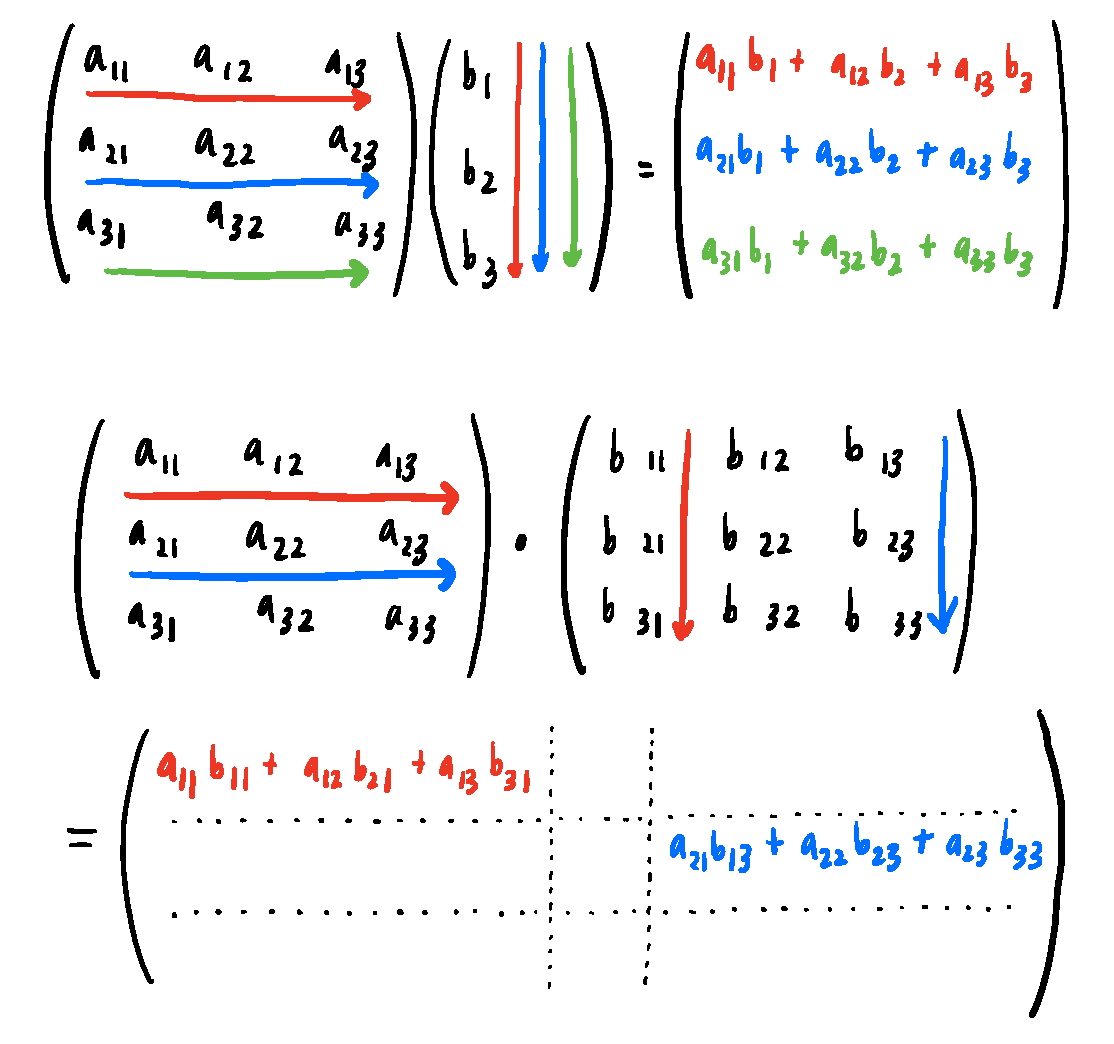
\includegraphics[width=\linewidth]{figs/matrixMult.pdf}
  \caption{Example matrix multiplication for $3\times 3$ matrices. {\it Top}: A
           matrix being applied to a 3D vector. {\it Bottom}: Multiplication of two
           matrices.}
  \label{fig:matrix}
\end{figure}

{\it Matrices} play a fundamental role in physics as well.
We will see they are very useful for understanding different kinds of
symmetries, but they have many other applications as well\footnote{For example
in quantum physics, you will eventually learn that measurable quantities can be
extracted as special, characteristic values of matrices. They can also be used
to solve systems of equations.}. Given a vector space $A^n$, we associate
$n\times n$ matrices\footnote{Such a matrix is usually called a {\it square
matrix}. Matrices don't have to be square matrices, i.e. they can have a
different number of rows than columns. In physics square
matrices matter the most, so that's all we'll worry about for these notes.}, 
which have the form
\begin{equation}\label{eq:basicMatrix}
  M=\left(\begin{array}{cccc}
          a_{11}   & a_{12} &       & a_{1n}\\
          a_{21}   & a_{22} &       & a_{2n}\\
                   &        & \ddots&       \\
          a_{n1}   & a_{n2} &       & a_{nn}
            \end{array}\right). 
\end{equation}
We call each entry $a_{ij}\in A$, $1\leq i,j\leq n$, an {\it element}. The position
of each element is indicated by two subscripts, the left
indicating the row number and the right indicating the column number.
Hence there are $n^2$ elements in a square matrix.

Matrices as defined above\footnote{That is, square matrices. By the way,
in this context of mapping vector spaces into themselves, we sometimes
call matrices {\it operators}\index{operator}.} map $A^n$ into itself, i.e.
\begin{equation}\label{eq:operatorDef}
  M:A^n\to A^n.
\end{equation}
In general, this mapping is achieved through matrix multiplication. If one
multiplies a vector $v$ with a matrix $M$, one gets for the $i\nth$ component
of the product $Mv$
\begin{equation}\label{eq:matTimesVec}
  (Mv)_i=\sum_{j=1}^n a_{ij}v_j,
\end{equation}
where $M$ is our matrix and $v$ is a vector. 

To understand the RHS of \equatref{eq:matTimesVec}, let's look at the example
\begin{equation}\label{eq:matTimesVecEx}
  \left(\begin{array}{cc}
          3   & 4\\ 
          5   & 6\\ 
            \end{array}\right)
  \colvec{2}{1}{-2}
  =\colvec{2}{b_1}{b_2}
\end{equation}
To get the first component of the product,
one starts with the first row of the matrix, multiplying the row's leftmost
element with the vector's first component. Then one adds the next-leftmost
element times the second component, and so on. To get the second component of
the product, one repeats using instead the second row of the matrix.
In our case, we obtain
\begin{equation}\begin{aligned}\label{eq:matMultEx}
  b_1 &= 3\times1 - 4\times2 = -5\\
  b_2 &= 5\times1 - 2\times6 = -7
\end{aligned}\end{equation}
See \figref{fig:matrix} (top) for
a colored representation of what this looks like for a $3\times3$ matrix
multiplying a vector in $\R^3$.

Eqs.~\eqref{eq:operatorDef} and \eqref{eq:matTimesVec} show us that one way to
look at matrices is as functions\footnote{In fact, this perspective is generally 
applicable any time one uses the words ``map" or ``mapping".} that take a vector 
and give back a vector.
For instance \equatref{eq:matMultEx} shows that the matrix in the LHS
of \equatref{eq:matTimesVecEx} maps
\begin{equation}
  \colvec{2}{1}{-2}
  \to\colvec{2}{-5}{-7}.
\end{equation}
Sometimes that perspective is useful, but it is often useful to think about
matrices as math objects in their own right. Matrices can, for instance, be added
together element-wise. 
\begin{equation}\begin{aligned}
  \left(\begin{array}{cccc}
          a_{00}   & a_{01} &       & a_{0n}\\ 
          a_{10}   & a_{11} &       & a_{1n}\\
                   &        &\ddots & \\
          a_{n0}   &        &       & a_{nn} 
  \end{array}\right)
  &+\left(\begin{array}{cccc}
          b_{00}   & b_{01} &       & b_{0n}\\ 
          b_{10}   & b_{11} &       & b_{1n}\\
                   &        &\ddots & \\
          b_{n0}   &        &       & b_{nn} 
  \end{array}\right)\\
  &=\left(\begin{array}{cccc}
          a_{00}+b_{00}   & a_{01}+b_{01} &        & a_{0n}+b_{0n}\\ 
          a_{10}+b_{10}   & a_{11}+b_{11} &        & a_{1n}+b_{1n}\\ 
                          &               & \ddots & \\
          a_{n0}+b_{n0}   &               &        & a_{nn}+b_{nn} 
  \end{array}\right)
\end{aligned}\end{equation}
Analogously as with many kinds of number systems, it is useful to introduce
in $n$ dimensions an additive identity\index{identity!additive} or zero matrix as
\begin{equation}
  \zd_n=\left(\begin{array}{cccc}
          0   & 0 &       & 0\\
          0   & 0 &       & 0\\
              &   & \ddots& \\
          0   &   &       & 0
            \end{array}\right), 
\end{equation}
i.e. it's the $n\times n$ matrix with 0 in every element. With our definition
of matrix addition, we find that for any $n\times n$ matrix $M$
\begin{equation}
\zd_n+M=M+\zd_n=M.
\end{equation}

Besides addition, it is useful to be able to carry out multiplication.
The simplest kind is scalar multiplication\index{multiplication!scalar},
which is defined similarly as with vectors. In particular if $\alpha\in A$,
then
\begin{equation}
  \alpha\left(\begin{array}{cccc}
          a_{00}   & a_{01} &       & a_{0n}\\ 
          a_{10}   & a_{11} &       & a_{1n}\\
                   &        &\ddots & \\
          a_{n0}   &        &       & a_{nn} 
  \end{array}\right)\equiv
  \left(\begin{array}{cccc}
          \alpha a_{00}   & \alpha a_{01} &       & \alpha a_{0n}\\ 
          \alpha a_{10}   & \alpha a_{11} &       & \alpha a_{1n}\\
                          &               &\ddots &  \\
          \alpha a_{n0}   &               &       & \alpha a_{nn} 
  \end{array}\right).
\end{equation}
One can also multiply a matrix $M$ and a matrix $L$. If $L$ has elements
$b_{ij}$, then the product $ML$ is defined element-wise by
\begin{equation}
  (ML)_{ij}=\sum_{k=1}^n a_{ik}b_{kj}.
\end{equation}
Again, this is not particularly easy\footnote{If you still found this explanation confusing, 
this \href{https://youtu.be/kT4Mp9EdVqs}{Khan academy tutorial}
may help.}
to read, so I show this visually for 3 dimensions in
\figref{fig:matrix} (bottom). 
You may be inclined to think that the above 
{\it matrix multiplication}\index{multiplication!matrix} behaves like normal
multiplication, but that is not the case. Most notably, it is not 
in general commutative.
For example
\begin{equation}
  \left(\begin{array}{cc}
          1   & 0\\ 
          0   & 0\\ 
            \end{array}\right)
  \left(\begin{array}{cc}
          0   & 1\\ 
          0   & 0\\ 
            \end{array}\right)
  =\left(\begin{array}{cc}
          0   & 1\\ 
          0   & 0\\ 
            \end{array}\right)
\end{equation}
but
\begin{equation}
  \left(\begin{array}{cc}
          0   & 1\\ 
          0   & 0\\ 
            \end{array}\right)
  \left(\begin{array}{cc}
          1   & 0\\ 
          0   & 0\\ 
            \end{array}\right)
  =\left(\begin{array}{cc}
          0   & 0\\ 
          0   & 0\\ 
            \end{array}\right).
\end{equation}

Again to continue our analogy with other number systems,
we introduce a multiplicative identity for matrices.
In $n$ dimensions, the {\it identity matrix} is
\begin{equation}
  \id_n=\left(\begin{array}{cccc}
          1   & 0 &       & 0\\
          0   & 1 &       & 0\\
          0   &   & \ddots& \\
          0   &   &       & 1
            \end{array}\right), 
\end{equation}
i.e. it is the matrix with 1 along the diagonal and 0 everywhere else. Using
matrix multiplication you can show that for any $n\times n$ matrix $M$
\begin{equation}
  M\id_n =\id_n M = M.
\end{equation}
That is to say, no matter which way you multiply a matrix by $\id_n$, 
you will always get the matrix back. 
%This may seem trivial, but the concept of the
%identity matrix is important and is used extensively in linear algebra. For
%example, it can be used to describe the standard basis which you can then use to
%define linear transformations. You don't need to know what all that is right
%now, but I want to drive home that we are introducing these definitions now to
%build on them later.
Sometimes a matrix is {\it invertible}, i.e. $\Exists M^{-1}$ so that
\begin{equation}
  M^{-1} M=\id_n. 
\end{equation}
We will not discuss strategies for matrix inversion in these short notes, but
finding matrix inverses, and indeed sometimes determining whether a matrix has
an inverse at all, is a topic deserving of a chapter on its 
own\footnote{In fact, some of the most important problems supercomputers work
on revolve around inverting matrices. For example, many machine learning
algorithms require the inversion of large matrices. In the context
of physically realistic lattice calculations, extremely large matrices must be
inverted many, many times to generate space-time snapshots and to measure
certain observables.}. 

Using the above definitions, one can show that for $\alpha,\beta\in A$
and $n\times n$ matrices $O$, $L$ and $M$ that
\begin{equation}\begin{aligned}
(\alpha+\beta)M&=\alpha M+\beta M,\\
\alpha(L+M)&=\alpha L+\alpha M,\\
L+M&=M+L,\\
O+(L+M)&=(O+L)+M.
\end{aligned}\end{equation}
These are most of the usual properties of being distributive, associative,
and having additive commutativity.
Again, importantly, matrix multiplication is in the general case not
commutative.\index{distributive}\index{associative}\index{commutative}

To round out this discussion of thinking about matrices as math objects in their
own right, it is sometimes useful to define functions of matrices.
For starters, we can always
raise a matrix to an arbitrary power $k\in\N$. Hence we have well defined
functions of the form
\begin{equation}
f(M)=M^k\equiv\underbrace{M\,M\,...\,M}_{k\text{ times}},
\end{equation}
and as with ordinary numbers, we define $M^0\equiv \id_n$.
Using scalar multiplication and matrix addition, we are therefore also
able to sensibly define polynomials of matrices
\begin{equation}
f(M)=\alpha_0\id_n + \alpha_1 M + \alpha_2 M^2...+\alpha_n M^n.
\end{equation}
The fact that we can construct polynomials out of matrices empowers us
to define even more general functions through their Taylor series.
For example, the exponential $\exp:\R\to\R$ is given through its Taylor expansion
as
\begin{equation}
\exp(x)=\sum_{i=0}^\infty \frac{x^k}{k!}.
\end{equation}
This allows us to define the exponential of a matrix as
\begin{equation}\label{eq:expMat}
\exp(M)=\sum_{i=0}^\infty \frac{M^k}{k!}.
\end{equation}
All the typical elementary functions $\sin$, $\sinh$, and so on can be
analogously defined on matrices.

Finally, I am obligated to introduce some notation one frequently encounters
in physics with regard to matrices. The {\it trace}\index{trace} of an 
$n\times n$ matrix is the sum of its diagonal elements,
\begin{equation}
  \tr M=\sum_i^nM_{ii}.
\end{equation}
When you {\it transpose}\index{transpose} a matrix, you interchange all of its
off-diagonal elements; i.e. the $i,j$-element gets replaced with the
$j,i$-element, and vice-versa. For example the transpose $M^t$ of the matrix in
\equatref{eq:basicMatrix} is given by
\begin{equation}
  M^t=\left(\begin{array}{cccc}
          a_{11}   & a_{21} &       & a_{n1}\\
          a_{12}   & a_{22} &       & a_{n2}\\
                   &        & \ddots&       \\
          a_{1n}   & a_{2n} &       & a_{nn}
            \end{array}\right). 
\end{equation} 
The {\it complex conjugate}\index{complex conjugate} 
of a matrix simply conjugates all its elements, i.e.
\begin{equation}
  M^*=\left(\begin{array}{cccc}
          a_{11}^*   & a_{12}^* &       & a_{1n}^*\\
          a_{21}^*   & a_{22}^* &       & a_{2n}^*\\
                     &          & \ddots&         \\
          a_{n1}^*   & a_{n2}^* &       & a_{nn}^*
            \end{array}\right). 
\end{equation}
Finally we will sometimes need the conjugate-transpose or 
{\it adjoint}\index{adjoint} of a matrix, which is indicated with a 
little dagger\footnote{Hence we sometimes say ``$M$-dagger".},
$M^\dagger$. It is
\begin{equation}
M^\dagger\equiv (M^*)^t.
\end{equation}
A matrix is said to be {\it unitary}\index{unitary} if
\begin{equation}
M^\dagger M=MM^\dagger=\id_n,
\end{equation}
i.e. unitary matrices are those whose inverses are the same as 
their adjoints.

\section{Calculus with many variables}

In your first encounter with calculus, you likely considered
functions that accept a single real number and then
produce a real number, i.e. functions
\begin{equation}
f:\R\to\R.
\end{equation}
Indeed, this is likely how you have looked at functions for the
majority of your mathematical career. However, a function can also consist of
many real inputs which produce many real outputs. Multivariable calculus is then
the generalization of calculus, where functions can
accept a list of numbers.
Formally\footnote{For example the function $f:\R^2\to\R$
maps a point on the 2-$d$ plane to a point on the number line.}, 
we allow 
\begin{equation}
f:\R^n\to\R,
\end{equation}
where $n\in\N$.
We want to gain some intuition about what it means to take derivatives
of $f$ and to integrate it.

Suppose for a moment we fix $y$, i.e. we don't let $y$ change. This defines a
new function $g$
\begin{equation}\label{eq:fixG}
g(x)\equiv f(x,y)\,\suchthat\text{ $y$ is held constant}.
\end{equation}
Since $g$ is now a function of $x$ only, we can take a derivative\footnote{I'm
being a bit hand-wavy here. It is of course important that your function behaves
nicely in a particular way that you will learn when you take a course in
multivariable calculus. In these notes we will assume the functions we deal with
can be differentiated or integrated unless otherwise stated.} w.r.t. 
$x$ in the familiar way. This defines the {\it partial derivative of $f$ with
respect to $y$}\index{partial derivative}:
\begin{equation}\label{eq:pdv}
\pdv{f(x,y)}{x}\equiv\frac{\dd g(x)}{\dd x}.
\end{equation}
Sometimes as shorthand we write $\partial_x f$ to indicate the above derivative. 
The partial derivative thus effectively treats $y$ as
if it were just another constant. 
Hence partial derivative isolates $x$ to see how $f$
changes when you vary $x$ alone\footnote{It is important for this kind of
thinking that there is no hidden dependence between $x$ and $y$. If $y=h(x)$ one
has to keep track of that, and be a bit careful.}. This is a crucial
manipulation to be able to do in the context of an experiment: One can imagine
having many knobs to turn and wanting to understand to effect of turning each of
them.

Let's try to understand this through a simple example, 
the function $z(x,y)=x^{2}+xy+y^{2}$. It has two inputs, $x$ and $y$. Both $x$ and
$y$ have some impact on the final output $z$. By taking the derivative
$\partial_x z=2x+y$, we learn how $x$
affects $z$ while not allowing $y$ to change.
A plot of $z$ as a function of $x$ and $y$
is shown as the blue surface in \figref{fig:partial_derivative}.
The red line indicates $z$ when we fix $y=1$. At $y=1$,
$\partial_x z(x)$ then corresponds to a tangent line to
the red curve at $x$.

\begin{figure}
  \centering
  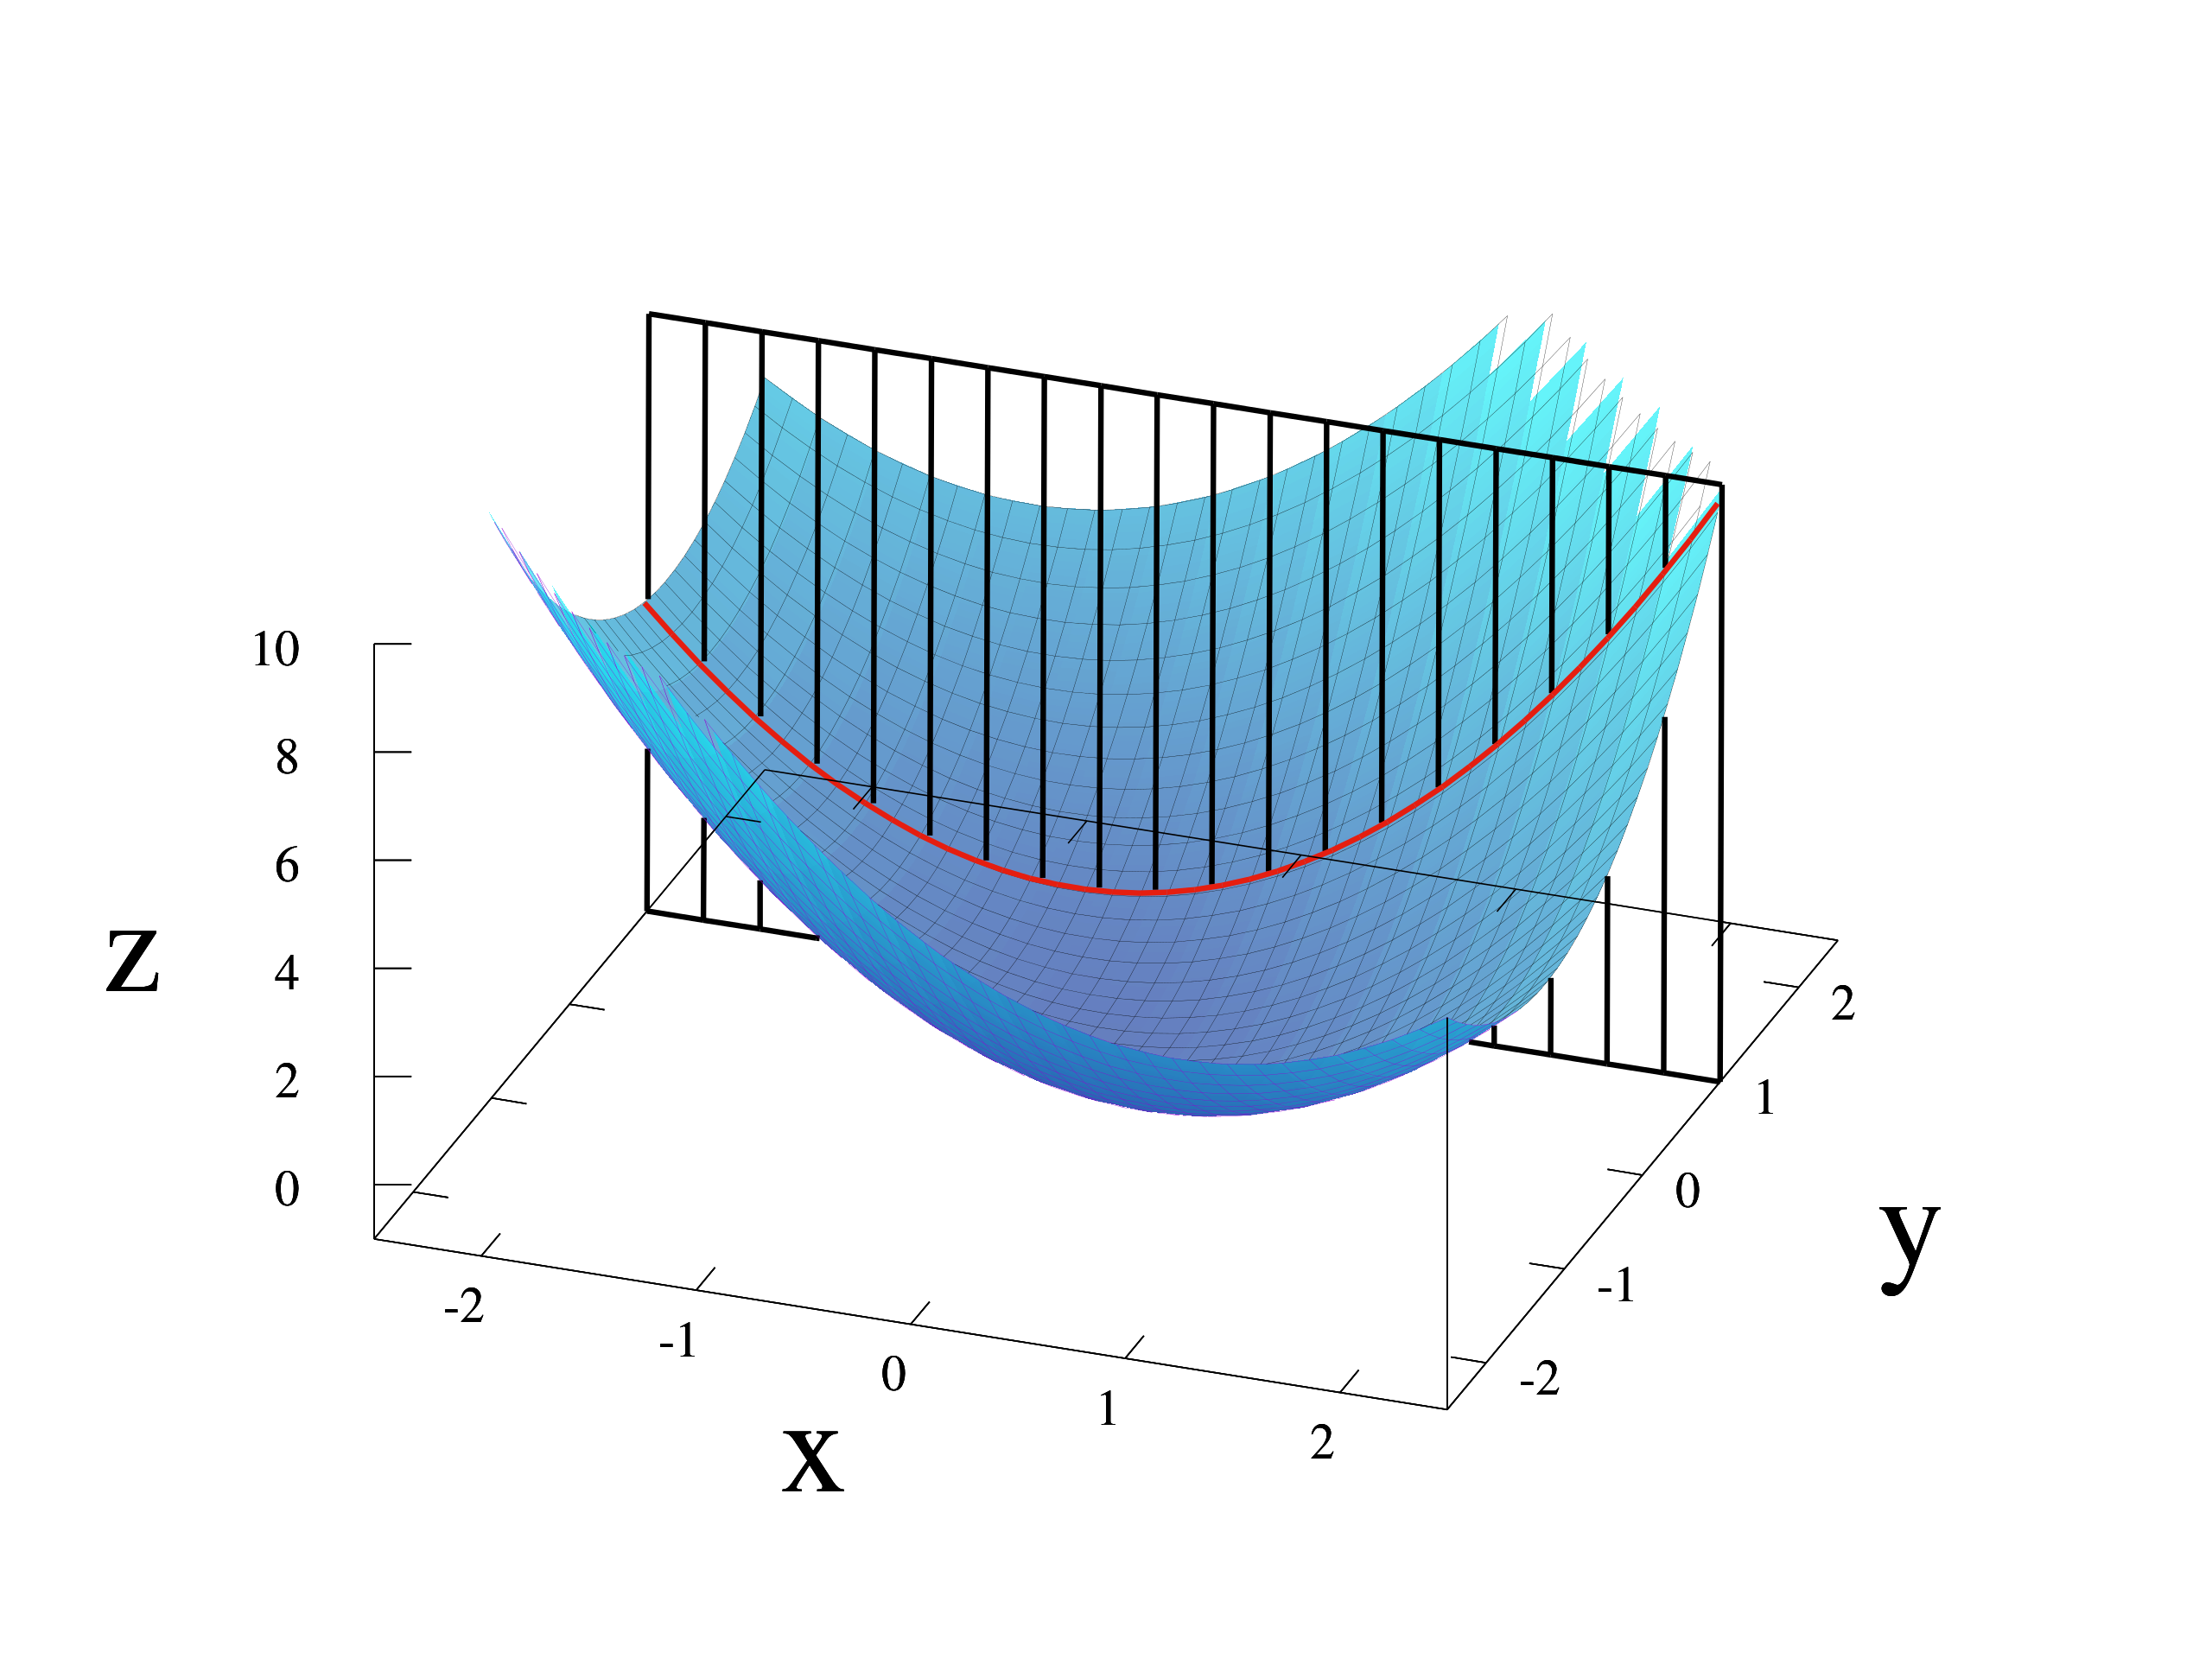
\includegraphics[width=\linewidth]{figs/Partial_func_eg.png}
  \caption{A graph of $z = x^2 + xy + y^2$, as well as the curve
  $z=x^2+x+1$ that results from fixing $y=1$.
  Image taken from Wikipedia~\cite{wiki:partial_derivative}.}
  \label{fig:partial_derivative}
\end{figure}

One can do the same thing holding $x$ fixed and taking a derivative
w.r.t. $y$; this procedure similarly defines a partial derivative w.r.t. 
$y$, $\partial_y f$.
We can generalize this to an arbitrary number of independent variables. 
For example for functions defined in four dimensions, we have a
function $f:\R^4\to\R$ of variables $x_1$, $x_2$, $x_3$, and $x_4$, which we
sometimes indicate\footnote{Similarly a function with a 3-$d$
domain may be indicated as $f(\vec{x})$.} as $f(\fvec{x})$. We define a 
function\footnote{This is simply abstracting our previous equation
\equatref{eq:fixG}. It is saying there is some
equation $g(x_\mu)$ ($\mu$ being one of $x_1$, $x_2$, $x_3$ or $x_4$) which is
equal to some more general equation $f(\fvec{x})$ where in $f(\fvec{x})$ the
variable $x_nu$ is held constant ($\nu$ being one of $x_1$, $x_2$, $x_3$, or
$x_4$ but it can't be the same as $\mu$).}
$g$
\begin{equation}
g(x_\mu)\equiv f(\fvec{x})\,
\suchthat\text{ $x_\nu$ is held constant $\Forall \nu\neq \mu$}
\end{equation}
where $1\leq\mu,\nu\leq4$. 
Then the partial derivative is
\begin{equation}
\pdv{f(\fvec{x})}{x_\mu}=\frac{\dd g(x_\mu)}{\dd x_\mu}.
\end{equation}
For shorthand, we use $\partial_\mu f$.

One further generalization to be made is to allow $f$ to map to a set besides
$\R$. For instance $f$ could be {\it vector-valued}\index{vector-valued} 
or {\it matrix-valued}\index{matrix-valued}, i.e. $f$ could output
vectors or matrices. 
%This can introduce some subtleties, and one may have to be even more careful. 
We won't
discuss these generalizations in these notes, but I just want you to know they
are possible and you will see them eventually.

Next let's discuss multiple integration. Again we start with a simple, 2-$d$
example. Suppose you have two integrable functions $f,g:\R\to\R$. Then by the
fundamental theorem of calculus, you know that when $a\leq x\leq b$.
\begin{equation}\label{eq:2dsimple}
\int_a^b\dd{x}f(x)=F(b)-F(a)~~~~\text{and}~~~~
\int_a^b\dd{x}g(x)=G(b)-G(a)
\end{equation}
for some functions $F$ and $G$, usually called {\it
primitives}\index{primitive}. Now imagine you encounter the product
\begin{equation}\label{eq:2dsimpleEval}
\int_a^b\dd{x}f(x)\int_a^b\dd{y}g(y).
\end{equation}
According to \equatref{eq:2dsimple}, this evaluates to
\begin{equation}
\left(F(b)-F(a)\right)\left(G(b)-G(a)\right).
\end{equation}
There, you just did you first 2-$d$ integral.

You may have noticed that I switched the variable name for $g$ from $x$ in
\equatref{eq:2dsimple} to $y$ in \eqref{eq:2dsimpleEval}. This is because in the
product, I want to notationally emphasize that the integrals are being evaluated
independently. This is no different from when wants to multiply two sums
\begin{equation}
  \sum_{i=1}^n f_i~~~~\text{and}~~~~\sum_{i=1}^n g_i.
\end{equation}
In order to keep track of the fact that the sums run over independent indices,
one writes the product\footnote{Sometimes we use the shorthand
$\sum_{i,j=1}^n$.} as
\begin{equation}
  \sum_{i=1}^n\sum_{j=1}^n f_ig_j.
\end{equation}
The product of integrals is no different, which makes sense if you think about
it since the integrals come from a limiting procedure starting with Riemann
sums. As long as the integration bounds are finite, we can utilize the fact
the order of symbols in the sum can be reorganized to reorganize symbols in the
integral. Hence \equatref{eq:2dsimpleEval} can be written as
\begin{equation}\label{eq:2dprodInt}
\int_a^b\int_a^b\dd{x}\dd{y}f(x)g(y)
=\int_a^b\int_a^b\dd{x}\dd{y}h(x,y),
\end{equation}
where $h(x,y)\equiv f(x)g(y)$. This logic is exactly how one can take the
integral of any function $h(x,y)$ in two dimensions, provided that $h$ can be
factorized into two functions $f$ and $g$ like that. 

%Said another way, we can
%express a function $h(x,y)$ as the product of the functions $f(x)$ and $g(y)$,
%i.e., $h(x,y) = f(x)g(y)$, then we can use the product rule of integration to
%evaluate the double integral of $h(x,y)$ over a region in the $x-y$ plane. The
%product rule of integration states that the double integral of a product of two
%functions $f(x)$ and $g(y)$ over a region $[a,b]\times[c,d]$ can be computed by
%integrating $f(x)$ over $[a,b]$ and $g(y)$ over $[c,d]$, and then multiplying
%the two results together. This is exactly what is done in Equation
%\eqref{eq:2dprodInt}, where we first integrate $f(x)g(y)$ with respect to $x$
%over the interval $[a,b]$, and then integrate the result with respect to $y$
%again over the interval $[a,b]$. This method can be used to evaluate the
%integral of function $h(x,y)$ that can be factorized into $f(x)$ and $g(y)$ like
%$h(x,y) = f(x)g(y)$.

% DC: I commented this out 1) because I'm not sure what is meant by "product rule
% of integration" and 2) because the rest is mostly a restating where the
% language isn't different enough to warrant repeating. I think the main issue
% is that I am not really describing multiple integration well, but I really
% want to avoid to get into the details on this, which will take quite a bit of
% space. I just want the reader to have a vague idea what I mean when I use a
% multiple-integral symbol, and nothing more. Maybe in a future edition I will
% set aside 10 or so pages to do treat it better.

Please note that in the general case, evaluating integrals 2-$d$ functions
is not quite that straightforward! Again, that above prescription only works
when $h$ can be factorized into two functions $f$ and $g$ of $x$ only and $y$
only. For instance it works when $h(x,y)=x^2\sin(y)$.
A function $h_{\text{tricky}}(x,y)=\sin(xy)$ will not integrate as a simple
product.
For now, I just want you to have some vague intuition what multiple integration
means, at least in some cases.
I foist the proper treatment of the general case of 2-$d$
integration onto your multivariable calculus professor.


The above procedure can be generalized to an arbitrary number of variables, as with
the partial derivative. In four dimensions, one encounters integrals like
\begin{equation}
\int_a^b\int_a^b\int_a^b\int_a^b
\dd{x_4}\dd{x_3}\dd{x_2}\dd{x_1}f(\fvec{x}).
\end{equation}
If at some point during the discussion we don't really care about the limits of
integration, we might write
\begin{equation}
\int\dd[4]{x}f(\fvec{x}),
\end{equation}
and if we want to limit the integration domain to some region $R$, for example a
hypersphere or something, we write
\begin{equation}
\int_R\dd[4]{x}f(\fvec{x}).
\end{equation}
Again, this business of shuffling around pieces of the integrand works if
it can be factorized into functions that each depend on one of the integration
variables only.
I just want you to have some intuition what is meant when a multiple integral
symbol appears.

\section{Probability and error}\label{sec:probAndError}

Crucial to the study of quantum physics, statistical physics, experiment, and
eventually lattice field theory is an understanding of probability and the
ability to understand statistics. These skills are actually quite important to
understand all modern science, not just physics, as well as in everyday
circumstances like politics\footnote{In this latter case it is of utmost
importance to understand these subjects to protect oneself against
misinformation. As Benjamin Disareli allegedly once said, ``There are lies,
damned lies, and statistics."}.
You already have a rough idea of probability: It's a way of saying whether you
think something will happen or not, while in general signaling that you aren't
completely certain. We will now make these ideas precise.

We will consider a {\it random variable}\index{random variable}\footnote{In this
section I will try to denote random variables by capital letters.} $X$ which
has some possible {\it outcomes}\index{outcome} $x_i$. The random variable will take 
one of the values in $x_i$, but we don't know for sure which one.
The set of all possible outcomes
\begin{equation}
  \Omega=\{x_1,x_2,...,x_N\},
\end{equation}
assuming there are $N\in\N$ possible outcomes, is called the {\it sample
space}\index{sample space}. If $|\Omega|$ is finite as in the above case, we
say that $X$ is {\it discrete}\index{discrete}. An {\it event}\index{event} $E$
is any subset of outcomes $E\subset\Omega$, and we assign it a {\it
probability}\index{probability} $\pr{E}$. Axiomatically speaking, the
probability has to fulfill two conditions:
\begin{enumerate}
  \item $\Forall E$, $0\leq\pr{E}\leq1$.
  \item $\pr{\Omega}=1$, i.e. the random variable $X$ needs to have some outcome
in $\Omega$. Another way to state this is that the probability of at least one
of the possibilities is 1. 
\end{enumerate}

Pragmatically you can assign a probability by repeating some experiment $n$
times. If the event $E$ occurs $N_E$ times, then
\begin{equation}
  \pr{E}\equiv\lim_{N\to\infty}\frac{N_E}{N}.
\end{equation}
Alternative, you can make some theoretical assignment of probabilities to
events. For instance when one tosses a coin, if one has no reason to believe the
coin is biased, it must be that
\begin{equation}
\pr{\text{heads}}=\pr{\text{tails}}=\frac{1}{2}.
\end{equation}
This theoretical assignment is nice, but it should eventually be checked against
some observation or measurement as well.

To be quantitative, we like to somehow map the possible outcomes to numbers. For
instance a die roll can be mapped to the set $\{1,2,3,4,5,6\}$. A reasonable
question to ask in this case is: If I toss a die, what can I expect? A measure
of this is the {\it expectation value}\index{expectation value}, which is
defined by
\begin{equation}
\ev{X}=\sum_{x\in\Omega}\pr{X=x}x,
\end{equation}
or more explicitly for the die,
\begin{equation}
\ev{\text{my die roll}}=\sum_{i=1}^6\frac{1}{6}\,i=3.5.
\end{equation}

Sometimes the cardinality of $\Omega$ is uncountably infinite. For instance you
may ask something like: What is the probability that a particle in this gas has
a speed between $v_1$ and $v_2$? In this case, the sample space is
\begin{equation}
  \Omega=\{x\suchthat0\leq x\leq c\},
\end{equation}
where $c$ is the speed of light\footnote{As we will reiterate in
\secref{sec:SR}, $c$ is the largest possible speed for anything.}.
In such a case we speak of a {\it continuous} random variable $X$.
The probability that $X$ takes any one particular value in $\Omega$ is
zero\footnote{Intuitively you could ask yourself: What is the probability that
my speed is exactly $\pi$ to all infinitely many digits? When checking against
experiment, you will never be able to resolve all infinitely many digits, so at
best you must specify a range corresponding to the resolution of your
instrument. In formal mathematical language, we require $\Omega$ to be
{\it measurable}.}. 
We can only assign
sensible probabilities to subsets of $\Omega$ of uncountably infinite
cardinality. In the above
case, this corresponds to the range of velocities between $v_1$ and $v_2$.
The probability that $X$ takes a value in the small range of velocities $\dd x$
is denoted
\begin{equation}
   \pr{X\in[x,x+\dd x]}=\dd{x}f(x),
\end{equation}
and hence for continuous random variables, the probability must instead
fulfill the properties
\begin{enumerate}
  \item  $0\leq\dd{x}f(x)\leq 1$ and
  \item $\int_{x\in\Omega}\dd{x}f(x)=1$.
\end{enumerate}
We call $f$ the {\it probability density function}\index{probability density
function} or PDF.
Correspondingly, the notion of an expectation value\index{expectation value}
must change as
\begin{equation}
\ev{X}=\int_{x\in\Omega}\dd{x}f(x)\,x.
\end{equation}
Meanwhile the {\it cumulative distribution function} (CDF) is the function
\index{CDF}
$F(x)$ given by
\begin{equation}
  F(x)\equiv \pr{X<x}=\int_{-\infty}^x\dd{t}f(t).
\end{equation} 



\begin{example*}{}{}
Two examples of important probability distributions include the {\it Gaussian}
or {\it normal} distribution,\index{PDF!normal}
\begin{equation}
  \gau(x,\hat{x},\sigma)\equiv\frac{1}{\sigma\sqrt{2\pi}}
  \exp\Bigg(-\frac{(x-\hat{x})^2}{2\sigma^2}\Bigg)
\end{equation}
where $\sigma$ is the standard deviation of the distribution and $\hat{x}$ is
the mean, and the {\it Cauchy} \index{PDF!Cauchy} distribution,
\begin{equation}
  \cau(x,\alpha)\equiv\frac{\alpha}{\pi\big(\alpha^2+x^2\big)}.
\end{equation}
I will refer to these special PDFs later, particularly the normal distribution.
I'll call their CDFs $\Gau$ and $\Cau$, respectively.
\end{example*}

From now on, we consider continuous random variables only.
Now that we know what probabilities and PDFs are, we can start thinking about
ways to characterize them. For example we can think about typical values taken
by a random variable from some distribution. We can get some information
from the mean and variance of a distribution. These are
both special cases of a more general concept.
In particular, let $n\in\N$.
  The {\it $n\nth$ moment} \index{moment}of the distribution $f(x)$ is
  \begin{equation}\label{dfn:mom}
    \ev{X^n}=\int_{-\infty}^\infty\dd{x}x^nf(x).
  \end{equation}

The mean and variance are the special cases $\hat{x}=\ev{X}$ and
$\sigma^2=\ev{(X-\hat{x})^2}$. Sometimes we call the mean the {\it expected
value}\index{expected value} or {\it expectation value}\index{expectation
value}, and sometimes we denote the variance $\variance$. Note that not all
probability distributions have well-defined moments. The Cauchy distribution is
very ill-behaved in this regard, since its $n\nth$ moment diverges
$\Forall n\in\N$.
Generally in the lab, one draws random variables from distributions
about which one has no a priori knowledge. Therefore in principle one
doesn't know the true moments these distributions. The
definition \eqref{dfn:mom} suggests a way to estimate them.
Suppose you draw a sample $X_1,...,X_N$:
  An {\it estimator}\index{estimator} of the $n\nth$ moment, $n\in\N$, is
  \begin{equation}
    \bar{X}^n\equiv\frac{1}{N}\sum_{i=1}^N X_i^n.
  \end{equation}
In the case $n=1$ we obtain the ordinary arithmetic average.
We use the hat to distinguish true values from estimators, which will
generally be denoted with a bar. For estimators of moments besides the
mean, we must be more careful.

Consider two intervals $[a,b]$ and $[c,d]$ and two random variables
$X$ and $Y$ drawn from PDFs $f$ and $g$, respectively. Then $X$ and $Y$ are
said to be {\it independent}\index{random variable!independent} if
\begin{equation}\label{dfn:ind}
  \pr{X\in[a,b]\text{ and }Y\in[c,d]}=\int_a^b\int_c^d\dd{x}\dd{y}f(x)\,g(y)
\end{equation}
Hence we see that the {\it joint PDF}\index{PDF!joint} of $X$ and $Y$
is $f(x)g(y)$. On the other hand, we say $X$ and $Y$ are {\it uncorrelated}
\index{random variable!uncorrelated} if
\begin{equation}
  \ev{XY}=\ev{X}\ev{Y},
\end{equation}
The {\it covariance}\index{covariance}
\begin{equation}\label{dfn:cov}
  \Cov[X,Y]\equiv\ev{XY}-\ev{X}\ev{Y}
\end{equation}
can be used to give a measure of how correlated $X$ and $Y$ are, or
one can use the {\it correlation}\index{correlation}
\begin{equation}\label{dfn:cor}
  \rho(X,Y)=\frac{\Cov[X,Y]}{\sqrt{\sigma^2_X\sigma^2_Y}}.
\end{equation}
So equivalently we say $X$ and $Y$ are correlated if $\rho(X,Y)=0$.
It's worth emphasizing that if $X$ and $Y$ are independent,
it follows that they are uncorrelated. This can be seen by applying
definition \eqref{dfn:mom} to the random variable $XY$, then using
definition \eqref{dfn:ind}. However if $X$ and $Y$ are
uncorrelated, {\it they can still be dependent}.
\begin{example*}{}{}
  Here's an extreme example by Cosma Shalizi~\cite{cosma_indep}.
Let $X$ be uniformly distributed
  on [-1,1] and let $Y=|X|$. Then clearly $Y$ depends on $X$. However it
  is easy to see that $Y$ is uniform on [0,1] and $\ev{XY}=0=\ev{X}\ev{Y}$.
  Hence $X$ and $Y$ are not correlated.
\end{example*}

The next two propositions show us how to add expectation values and
random variables. Let $X$ and $Y$ be independent random variables
drawn from PDFs $f$ and $g$, respectively.
\begin{proposition}{}{}
  Let $a,b\in\R$ be constants. Then
  $$\ev{aX+bY}=a\ev{X}+b\ev{Y}.$$
  \begin{proof}
    Since $X$ and $Y$ are independent, their joint PDF is $fg$. Then
    \begin{equation*}
      \begin{aligned} 
      \ev{aX+bY}&=\int\dd{x}\dd{y}(ax+by)f(x)g(y)\\
                &=a\int\dd{x}\dd{y}x\,f(x)g(y)+
                 b\int\dd{x}\dd{y}y\,f(x)g(y)\\
                &=a\int\dd{x}x\,f(x)+b\int\dd{y}y\,g(y)\\
                &=a\ev{X}+b\ev{Y}.
      \end{aligned}
    \end{equation*}
  \end{proof}
\end{proposition}

\begin{proposition}{}{addvars}
  The PDF of the random variable $Z=X+Y$ is given by the convolution
  \begin{equation*}
    h(z)=\int_{-\infty}^\infty\dd{x}f(x)g(z-x)
  \end{equation*}
  \begin{proof}
    The CDF of $Y$ is, according to \equatref{dfn:ind},
    \begin{equation*}
      H(y)=\int_{x+y\leq z}\dd{x}\dd{y}f(x)g(y)
          =\int_{-\infty}^\infty\dd{x}f(x)\int_{-\infty}^{z-x}
            \dd{y}g(y).
    \end{equation*}
    The PDF $h$ follows from the Fundamental Theorem of Calculus:
    \begin{equation*}
      h(z)=\dv{H}{z}=\dv{H}{(z-x)}
          =\int_{-\infty}^\infty\dd{x}f(x)g(z-x).
    \end{equation*}
  \end{proof}
\end{proposition}


\subsection{The normal distribution}
\index{PDF!normal}
Now we're going to focus on results about the normal distribution specifically.
This first proposition will aid us in some of the calculations.

\begin{proposition}{}{gauss}
  Let $\alpha>0$. Then
  \begin{equation*}
    \int_{-\infty}^\infty\dd{x}e^{-\alpha x^2}=\sqrt{\frac{\pi}{\alpha}}.
  \end{equation*}
  \begin{proof}
    The trick is to just square the LHS:
    \begin{equation*}\begin{aligned}
      \left(\int_{-\infty}^\infty\dd{x}e^{-\alpha x^2}\right)^2
      &=\int_{-\infty}^\infty\int_{-\infty}^\infty\dd{x}\dd{y}
        e^{-\alpha(x^2+y^2)}\\
      &=\int_0^\infty \dd{r}r\int_0^{2\pi}\dd{\theta}e^{-\alpha r^2}\\
      &=\frac{\pi}{\alpha}.
    \end{aligned}\end{equation*}
  \end{proof}
\end{proposition}

For the next result
let $X_1$ and $X_2$ be two independent random variables drawn from normal
distributions with respective means $\hat{x}_1$ and $\hat{x}_2$ and
standard deviations $\sigma_1$ and $\sigma_2$.
\begin{proposition}{}{addgauss}
  The random variable $Y=X_1+X_2$ is normally distributed with mean
  $\hat{x}_1+\hat{x}_2$ and variance $\sigma_1^2+\sigma_2^2$.
  \begin{proof}
    By \propref{prp:addvars}, the sum $Y$ has the distribution
    \begin{equation*}
      g(y)=\frac{1}{2\pi\sigma_1\sigma_2}
           \int_{-\infty}^\infty\dd{x}\exp\left[
             -\frac{(x-\hat{x}_1)^2}{2\sigma_1^2}
             -\frac{(y-x-\hat{x}_2)^2}{2\sigma_2^2}\right].
    \end{equation*}
    Pull everything out of the integral that doesn't depend on $x$,
    then complete the square with what's left over.
    One obtains for $g(y)$
    $$
      \frac{1}{2\pi\sigma_1\sigma_2}
           \exp\left[-\frac{(y-\hat{x}_1-\hat{x}_2)^2}
                      {2(\sigma_1^2+\sigma_2^2)}\right]
           \int_{-\infty}^\infty\dd{x}
           \exp\left[-\frac{\sigma_1^2+\sigma_2^2}
                     {2\sigma_1^2\sigma_2^2}(x+C)^2\right],
    $$
    where $C$ is just a bunch of stuff that doesn't depend on $x$.
    Therefore you can make the substitution $u=x+C$ with $\dd u=\dd x$ and
    carry out the new integral using \propref{prp:gauss}.
    The result is
    \begin{equation*}
      g(y)=\frac{1}{\sqrt{2\pi(\sigma_1^2+\sigma_2^2)}}
           \exp\left[-\frac{(y-\hat{x}_1-\hat{x}_2)^2}
                      {2(\sigma_1^2+\sigma_2^2)}\right].
    \end{equation*}
  \end{proof}
\end{proposition}

Since the normal distribution is so important, so must be its CDF.
Unfortunately the integral of the normal PDF is {\it non-elementary};
\index{non-elementary} that is, it can't be expressed in terms of
polynomials or standard
functions like $\sin$, $\cos$, or $\exp$. Therefore we give a name
to this special function.
The {\it error function}\index{error function} is
\begin{equation}
  \erf(x)\equiv\frac{2}{\sqrt{\pi}}\int_0^x\dd{t}e^{-t^2}.
\end{equation}
Then we can write the Gaussian CDF with mean 0 as
\begin{equation}
  \label{eq:gaussCDF}
  \Gau(x,0,\sigma)=\frac{1}{\sqrt{2\pi}\sigma}
                   \int_{-\infty}^x\dd{t}e^{-t^2/2\sigma^2}
                  =\frac{1}{2}+\frac{1}{2}
                   \erf\left(\frac{x}{\sqrt{2}\sigma}\right).
\end{equation}
Now we can list some pretty powerful applications of the normal distribution.
For instance one often must compare two empirical estimates of some mean.
Usually these estimates are different, and one might wonder whether this
disparity is real or just plain unlucky. More precisely:
\index{Gaussian difference test}
\begin{theorem}{Gaussian difference test}{}\label{thm:gaudif}
  Suppose $\bar{X}$ and $\bar{Y}$ are correct estimates of
  some expectation
  value, i.e. they are normally distributed with the same mean, and call
  their respective standard deviations $\sigma_X$ and
  $\sigma_Y$. Then the probability that $\bar{X}$
  and $\bar{Y}$ differ by at least $D$ is
  \begin{equation*}
    \pr{|\,\bar{X}-\bar{Y}|>D}=1-\erf\left(\frac{D}
       {\sqrt{2(\sigma_X^2+\sigma_Y^2)}}\right).
  \end{equation*}
  \begin{proof}
    From \propref{prp:addgauss}, the random variable
    $\bar{X}-\bar{Y}$ is normally distributed with mean 0
    and variance $\sigma_D^2=\sigma_X^2+\sigma_Y^2$. Therefore by
    \equatref{eq:gaussCDF}, the probability that $\bar{X}$ and
    $\bar{Y}$ are at most $D$ apart is
    \begin{equation*}
      \begin{aligned}
        \pr{|\,\bar{X}-\bar{Y}|<D}
            &=\pr{-D<\bar{X}-\bar{Y}<D}\\
            &=\Gau(D,0,\sigma_D)-\Gau(-D,0,\sigma_D)\\
            &=1-2\Gau(-D,0,\sigma_D)\\
            &=\erf\left(\frac{D}{\sqrt{2}\sigma_D}\right).
      \end{aligned}
    \end{equation*}
    And of course, $\pr{|\,\bar{X}-\bar{Y}|>D}
     =1-\pr{|\,\bar{X}-\bar{Y}|<D}$.
  \end{proof}
\end{theorem}
In other words, the above theorem gives the probability that the
observed difference $|\bar{X}-\bar{Y}|$ is due to chance. This probability
is called the \index{q-value}{\it q-value}. In practice one sets some
threshold on $q$ below which one investigates further whether the
underlying distributions of the estimates are different. Often one
takes the threshold as 0.05.

Finally, suppose you're an experimenter taking independent measurements of
some observable. Furthermore suppose you don't know anything about the
observable, except that it comes from some distribution with finite variance.
The central limit theorem (CLT) says that armed with this information alone,
you know that the sample mean will be normally distributed about
the true mean. Here is the precise statement.\index{Central limit theorem}
\begin{theorem}{Central limit theorem}{}
  Let $X_1,...,X_N$ be $N$ independent random variables drawn from PDF $f$.
  Suppose further that $f$ has mean $\hat{x}$ and variance $\sigma^2$.
  Then the PDF of the estimator $\bar{X}$ converges to
  $\gau(\bar{X},\hat{x},\sigma/\sqrt{N})$.
\end{theorem}
The only proof of this theorem I'm aware of requires the introduction of
{\it characteristic functions}, which I would like to avoid. So I will ask you
to trust this theorem. The central limit theorem tells you that, if you have
some experiment you repeat $N$ times, the arithmetic mean $\bar{X}$ is likely to
be only $\sigma/\sqrt{N}$ away from the true mean $\hat{x}$. As you increase
$N$, this statement becomes more tight, which corresponds to the intuition that
as you repeat an experiment more and more times, you have a more and more exact
understanding of things.
More specifically, for large enough $N$, we expect the true mean to be within
$\sigma/\sqrt{N}$ of the estimator roughly 68\% of the time.
\tabref{tab:normal} gives the area under a Gaussian curve
for different numbers of standard deviations away from the mean.

\begin{table}
\centering
\caption{Table of areas under the curve for the normal distribution.
The last column gives the probability that a random variable
drawn from the distribution falls at least the given number of error bars
away from the mean.}
\begin{tabularx}{\linewidth}{cCr}
\hline\hline
Number of $\sigma$ from $\hat{x}$ & Area under curve & About 1 in ...\\
\hline
1 & 0.682 689 49 & 3\\
2 & 0.954 499 74 & 22\\
3 & 0.997 300 20 & 370\\
4 & 0.999 936 66 & 15 787\\
5 & 0.999 999 43 & 1 744 278\\
\hline\hline
\end{tabularx}
\label{tab:normal}
\end{table}



\section{Groups}

Very roughly, a group is a set with a rule that lets you combine two group
elements to make a new one. More precisely, 
a {\it binary operation} \index{binary operation} $\bullet$ on a set 
$G$ is a function $\bullet : G\times G\to G$. A {\it group} \index{group}
 is a set $G$ equipped with a binary operation $\bullet$ that satisfies 
the following axioms:
  \begin{enumerate}
    \item $\bullet$ is associative.
    \item $\Exists \id \in G\suchthat\Forall g \in G$, 
          \begin{equation}
            \id\bullet g=g\bullet \id=g. 
          \end{equation} This element $\id$ is called the {\it identity}.
          \index{identity}
    \item $\Forall g \in G,~\Exists g^{-1} \in G$, called the 
          {\it inverse} \index{inverse} of $g$, such that
          \begin{equation}
            g^{-1}\bullet g=g\bullet g^{-1}=\id.
          \end{equation}
  \end{enumerate}
If group elements commute under $\bullet$ the group is said to be
{\it abelian}\index{abelian}. The {\it order} \index{order} of a group, 
denoted $|G|$, is its cardinality. A {\it subgroup} \index{subgroup}
$H$ of $G$ is a non-empty subset of $G$ that itself forms a group under 
$\bullet$ and in this case we will write\footnote{
It should be clear from context whether this symbol indicates group 
organization or magnitude.} 
$H\leq G$. 
%Finally a group is {\it cyclic} \index{cyclic}
%if it is generated by a single element; that is, if 
%$\Exists g\in G$ such that $G=\{g^{n}\suchthat  n\in\Z\}$.

It's not too common to write the
$\bullet$ explicitly when showing the composition of two elements. So for
example you will often see $gh$ as shorthand for $g\bullet h$. In general I will
only refer to operations on algebraic structures explicitly when giving the
definition of that structure. Therefore you can expect to see $gh$ instead of
$g\bullet h$ from here on out.

Here I want to prove a small fact about groups, just to give you an idea of how
such a proof would work. Basic facts about groups don't usually require any
tricks; you can usually just chase definitions.

\begin{proposition}{}{}
  A subset H of G is a subgroup of G if and only if
  $$a,b\in H\Rightarrow ab^{-1}\in H$$
  \begin{proof}
    ($\Rightarrow$) Follows immediately from the definition of a subgroup. To 
    show ($\Leftarrow$) let $b\in H$. Then by the above conditional, $bb^{-1}
    \in H$, which shows $\id\in H$. To show the existence of inverses in $H$, 
    note $\id,b\in H\Rightarrow \id b^{-1}\in H\Rightarrow b^{-1}\in H$. 
    Finally, associativity is inherited from G.
  \end{proof}
\end{proposition}

\begin{example*}{}{}
\begin{enumerate}
  \item $\Z,\ \Q,\ \R$, and $\C$ are all groups
        under addition, and
        $$ 
          \Z \leq \Q \leq \R \leq \C.
        $$ 
        Each of these sets with 0 removed could also form a group under
        multiplication.
  \item Sets of objects besides numbers also form groups. For example let $V$ 
        be any non-empty set of objects and let $S_{V}$ be the set of all
        permutations of $V$. Then $S_{V}$ forms a group under function
        composition called the {\it symmetric group}\index{group!symmetric} 
        on the set $V$.
\end{enumerate}
\end{example*}

\subsection{Why do groups matter in physics?}\label{sec:groupsMatter}

Besides the examples of groups discussed above, one common type of group is a
group of symmetries of some system. For example consider the circle of radius 1. 
All rotations in the plane of the circle are symmetries of the circle. 
Any point on the circle can be represented as a vector
\begin{equation}\label{eq:s}
\vec{s}=\colvec{2}{\cos\theta}{\sin\theta}, 
\end{equation}
where $0\leq\theta<2\pi$. Let
\begin{equation}\label{eq:rot}
R_\phi\equiv\left(\begin{array}{cc}
          \cos\phi   & -\sin\phi  \\
          \sin\phi   &  \cos\phi  \\
            \end{array}\right). 
\end{equation}
This matrix will rotate $\vec{s}$ by an angle $\phi$.
This can be seen by applying $R_\phi$ to $\vec{s}$ using matrix multiplication
and using some trig identities. More importantly the set
\begin{equation}
\U(1)=\{R_\phi\suchthat0\leq\theta<2\pi\}
\end{equation}
forms a group. This is sometimes called the\index{circle group} {\it circle
group} or the\index{unitary group} {\it unitary group of degree 1}\footnote{As
the name suggests, the matrix representation of this group can be shown to be
unitary as defined in \secref{sec:vecmat}.}.

Every finite group can be expressed using matrices.
A set of matrices that behave the same way as a group is called
a\index{matrix representation} {\it matrix representation}. Many infinite groups
also have matrix representations. Matrix representations are often useful to get
some intuition for how a group works. Equation~\eqref{eq:rot} effectively
summarizes a representation of $\U(1)$.

Symmetry groups, especially continuous symmetry groups like $\U(1)$, are of
utmost importance in physics. This was discovered by Emmy Noether in the early
1900s. We give a rough\footnote{I use the word ``system" here in an
intentionally vague way. The correct statement requires to introduce the {\it
action} of a system; then one is rather interested in symmetries of the action.
You will learn more about this as you continue in physics. I view this
discussion as too much detail for a first interaction with LFT.} 
statement of her theorem without proof, which again would
be a bit too much of a digression.
\begin{theorem}{Noether}{}
For every continuous symmetry of a system, there exists a corresponding 
conserved quantity.
\end{theorem}

The conserved quantity in Noether's theorem is called a\index{charge} {\it charge}.
This name is chosen purposefully: from the modern perspective of particle
physics, the electric charge is closely connected with the group $\U(1)$. 
Moreover a class of elementary particles, the so-called\index{boson} 
{\it gauge bosons}, are thought to be, in a sense, physical manifestations of
these symmetries. This suggests that the idea of a charge is more general than
just electric charge, and that other groups may correspond to other charges and
particles.


\subsection{Which groups will we care about?}

We are going to eventually investigate quantum chromodynamics (QCD), which describes
one corner of particle physics. There we will encounter a new charge called
{\it color}\footnote{Here the word color is used as an analogy. It has nothing
to do with visible light.}, and its corresponding symmetry group is the
{\it special unitary group of degree $N_c$}, $\SU(N_c)$, where $N_c$ is the number of
colors. In nature $N_c=3$, but it is sometimes of academic interest to consider
different numbers of colors.

The fact that $N_c=3$ is actually what led to the use of the
terminology\index{charge!color} ``color charge". Let's try to understand this. 
In electromagnetism (EM), there is only one kind of charge,
the\index{charge!electric} electric charge. It can be positive or negative. If I
would like to make an electric-charge-neutral state, I can accomplish this only
by adding as many positive charges as negative charges.
In QCD, there are three kinds of charges, which we sometimes call {\it red},
{\it green}, and {\it blue}. If I have a system with three particles, each
having respectively red, green, and blue color charge, I get a 
color-charge-neutral state. This color naming is thus a mnemonic, for if I mix
red, green, and blue paint, I get white paint.

So $\SU(3)$ will be the group we care about the most. Associated to this
symmetry group is, according to Noether, a conserved charge. This is the color
charge. The particle that we consider a physical manifestation of this symmetry
is the\index{gluon} {\it gluon}. The gluon is responsible for mediating one of
the fundamental forces, which we will discuss in more detail in \secref{sec:SM}.

\section{Further reading}

I have given an extremely superficial introduction to most of these subjects. If
you would like some additional resources, besides taking classes, I can suggest
a few books I found useful.
\begin{itemize}
  \item Rigorous single-variable calculus: 
{\it Calculus} by Michael Spivak~\cite{spivak08} is probably the best
introduction to real analysis that I have tried.
Rubin's {\it Principles of Mathematical Analysis}~\cite{rudin1976principles} is
at a much higher level and less pedagogical, but it does contain a construction
of $\R$ from $\Q$.
  \item Multivariable calculus: For doing practical calculations in one or more
variables I found 
{\it Calculus with Analytic Geometry} by Simmons~\cite{simmons1995calculus}
to be quite helpful.
  \item Linear algebra: Curtis's
{\it Linear Algebra: An Introductory Approach} is quite rigorous, but perhaps
not particularly helpful in building intuition. It's the only book I've tried. 
  \item Probability: I found
Feller's {\it An Introduction to Probability Theory and Its 
Applications}~\cite{feller1}
to be rigorous, readable, and full of fun problems.
  \item Group theory:
If you would like to understand group theory more deeply,
a really good, rigorous introduction to groups accessible to undergrads is 
Dummit and Foote~\cite{dummit_abstract_2004}. To learn about Lie groups
like $\SU(3)$, my personal favorite resource is Georgi~\cite{georgi_lie_1999}.
\end{itemize}
There are also books that try to capture large swathes of math methods in
physics. Probably the most popular is Arfken's {\it Mathematical Methods for
Physicists}~\cite{garfken67:math}.

\section*{Exercises}

\begin{enumerate} 
  \item Let $n\in\N$. Prove that vectors in $\R^n$ are associative, commutative,
        and distributive.
  \item Prove that $\id_n M=M$ for any $n\times n$ matrix $M$.
  \item If $M$ is invertible, will it commute with its inverse? Why or why not?
  \item Prove that $\Q$, $\R$, and $\C$ form groups under addition. Also
        prove it for multiplication.
  \item Show that $R_\phi$ defined in \equatref{eq:rot} rotates $\vec{s}$ defined
        in \equatref{eq:s} by $\phi$. {\it Hint}: You will eventually use some
        trigonometry identities.
  \item Show that $R_\phi$ is a unitary matrix.
  \item Prove that $\U(1)$ is a group.
\end{enumerate}


\bibliographystyle{unsrtnat}
\bibliography{bibliography}
 
